%%%%%%%%%%%%%%%%%%%%%%%%%%%%%%%%%%%%%%%%%
% Lachaise Assignment
% LaTeX Template
% Version 1.0 (26/6/2018)
%
% This template originates from:
% http://www.LaTeXTemplates.com
%
% Authors:
% Marion Lachaise & François Févotte
% Vel (vel@LaTeXTemplates.com)
%
% License:
% CC BY-NC-SA 3.0 (http://creativecommons.org/licenses/by-nc-sa/3.0/)
% 
% Modified:
% Basil Minkov
%%%%%%%%%%%%%%%%%%%%%%%%%%%%%%%%%%%%%%%%%

%----------------------------------------------------------------------------------------
%	PACKAGES AND OTHER DOCUMENT CONFIGURATIONS
%----------------------------------------------------------------------------------------

\documentclass[12pt,a4paper,oneside]{article}

\usepackage[utf8]{inputenc}
\usepackage[russian]{babel}
\usepackage{graphicx}
\usepackage{wrapfig}
\usepackage{float}
\usepackage{subcaption}
\usepackage[font=scriptsize]{caption}
\usepackage{xcolor}
\definecolor{mygray}{gray}{0.4}
\usepackage[top=2.5cm,bottom=2.5cm,right=2.5cm,left=2.5cm,bindingoffset=0cm]{geometry}
\usepackage[colorlinks=true, a4paper=true, pdfstartview=FitV,
linkcolor=black, citecolor=mygray, urlcolor=mygray]{hyperref}
% \usepackage{natbib}


%%%%%%%%%%%%%%%%%%%%%%%%%%%%%%%%%%%%%%%%%
% Lachaise Assignment
% Structure Specification File
% Version 1.0 (26/6/2018)
%
% This template originates from:
% http://www.LaTeXTemplates.com
%
% Authors:
% Marion Lachaise & François Févotte
% Vel (vel@LaTeXTemplates.com)
%
% License:
% CC BY-NC-SA 3.0 (http://creativecommons.org/licenses/by-nc-sa/3.0/)
% 
%%%%%%%%%%%%%%%%%%%%%%%%%%%%%%%%%%%%%%%%%

%----------------------------------------------------------------------------------------
%	PACKAGES AND OTHER DOCUMENT CONFIGURATIONS
%----------------------------------------------------------------------------------------

\usepackage{amsmath,amsfonts,stmaryrd,amssymb} % Math packages

\usepackage{enumerate} % Custom item numbers for enumerations

\usepackage[ruled]{algorithm2e} % Algorithms

\usepackage[framemethod=tikz]{mdframed} % Allows defining custom boxed/framed environments

\usepackage{listings} % File listings, with syntax highlighting
\lstset{
	basicstyle=\ttfamily, % Typeset listings in monospace font
}

%----------------------------------------------------------------------------------------
%	DOCUMENT MARGINS
%----------------------------------------------------------------------------------------

\usepackage{geometry} % Required for adjusting page dimensions and margins

\geometry{
	paper=a4paper, % Paper size, change to letterpaper for US letter size
	top=2.5cm, % Top margin
	bottom=3cm, % Bottom margin
	left=2.5cm, % Left margin
	right=2.5cm, % Right margin
	headheight=14pt, % Header height
	footskip=1.5cm, % Space from the bottom margin to the baseline of the footer
	headsep=1.2cm, % Space from the top margin to the baseline of the header
	%showframe, % Uncomment to show how the type block is set on the page
}

%----------------------------------------------------------------------------------------
%	FONTS
%----------------------------------------------------------------------------------------

\usepackage[utf8]{inputenc} % Required for inputting international characters
\usepackage[T1]{fontenc} % Output font encoding for international characters

\usepackage{XCharter} % Use the XCharter fonts

%----------------------------------------------------------------------------------------
%	COMMAND LINE ENVIRONMENT
%----------------------------------------------------------------------------------------

% Usage:
% \begin{commandline}
%	\begin{verbatim}
%		$ ls
%		
%		Applications	Desktop	...
%	\end{verbatim}
% \end{commandline}

\mdfdefinestyle{commandline}{
	leftmargin=10pt,
	rightmargin=10pt,
	innerleftmargin=15pt,
	middlelinecolor=black!50!white,
	middlelinewidth=2pt,
	frametitlerule=false,
	backgroundcolor=black!5!white,
	frametitle={Command Line},
	frametitlefont={\normalfont\sffamily\color{white}\hspace{-1em}},
	frametitlebackgroundcolor=black!50!white,
	nobreak,
}

% Define a custom environment for command-line snapshots
\newenvironment{commandline}{
	\medskip
	\begin{mdframed}[style=commandline]
}{
	\end{mdframed}
	\medskip
}

%----------------------------------------------------------------------------------------
%	FILE CONTENTS ENVIRONMENT
%----------------------------------------------------------------------------------------

% Usage:
% \begin{file}[optional filename, defaults to "File"]
%	File contents, for example, with a listings environment
% \end{file}

\mdfdefinestyle{file}{
	innertopmargin=1.6\baselineskip,
	innerbottommargin=0.8\baselineskip,
	topline=false, bottomline=false,
	leftline=false, rightline=false,
	leftmargin=2cm,
	rightmargin=2cm,
	singleextra={%
		\draw[fill=black!10!white](P)++(0,-1.2em)rectangle(P-|O);
		\node[anchor=north west]
		at(P-|O){\ttfamily\mdfilename};
		%
		\def\l{3em}
		\draw(O-|P)++(-\l,0)--++(\l,\l)--(P)--(P-|O)--(O)--cycle;
		\draw(O-|P)++(-\l,0)--++(0,\l)--++(\l,0);
	},
	nobreak,
}

% Define a custom environment for file contents
\newenvironment{file}[1][File]{ % Set the default filename to "File"
	\medskip
	\newcommand{\mdfilename}{#1}
	\begin{mdframed}[style=file]
}{
	\end{mdframed}
	\medskip
}

%----------------------------------------------------------------------------------------
%	NUMBERED QUESTIONS ENVIRONMENT
%----------------------------------------------------------------------------------------

% Usage:
% \begin{question}[optional title]
%	Question contents
% \end{question}

\mdfdefinestyle{question}{
	innertopmargin=1.2\baselineskip,
	innerbottommargin=0.8\baselineskip,
	roundcorner=5pt,
	nobreak,
	singleextra={%
		\draw(P-|O)node[xshift=1em,anchor=west,fill=white,draw,rounded corners=5pt]{%
		Question \theQuestion\questionTitle};
	},
}

\newcounter{Question} % Stores the current question number that gets iterated with each new question

% Define a custom environment for numbered questions
\newenvironment{question}[1][\unskip]{
	\bigskip
	\stepcounter{Question}
	\newcommand{\questionTitle}{~#1}
	\begin{mdframed}[style=question]
}{
	\end{mdframed}
	\medskip
}

%----------------------------------------------------------------------------------------
%	WARNING TEXT ENVIRONMENT
%----------------------------------------------------------------------------------------

% Usage:
% \begin{warn}[optional title, defaults to "Warning:"]
%	Contents
% \end{warn}

\mdfdefinestyle{warning}{
	topline=false, bottomline=false,
	leftline=false, rightline=false,
	nobreak,
	singleextra={%
		\draw(P-|O)++(-0.5em,0)node(tmp1){};
		\draw(P-|O)++(0.5em,0)node(tmp2){};
		\fill[black,rotate around={45:(P-|O)}](tmp1)rectangle(tmp2);
		\node at(P-|O){\color{white}\scriptsize\bf !};
		\draw[very thick](P-|O)++(0,-1em)--(O);%--(O-|P);
	}
}

% Define a custom environment for warning text
\newenvironment{warn}[1][Warning:]{ % Set the default warning to "Warning:"
	\medskip
	\begin{mdframed}[style=warning]
		\noindent{\textbf{#1}}
}{
	\end{mdframed}
}

%----------------------------------------------------------------------------------------
%	INFORMATION ENVIRONMENT
%----------------------------------------------------------------------------------------

% Usage:
% \begin{info}[optional title, defaults to "Info:"]
% 	contents
% 	\end{info}

\mdfdefinestyle{info}{%
	topline=false, bottomline=false,
	leftline=false, rightline=false,
	nobreak,
	singleextra={%
		\fill[black](P-|O)circle[radius=0.4em];
		\node at(P-|O){\color{white}\scriptsize\bf i};
		\draw[very thick](P-|O)++(0,-0.8em)--(O);%--(O-|P);
	}
}

% Define a custom environment for information
\newenvironment{info}[1][Info:]{ % Set the default title to "Info:"
	\medskip
	\begin{mdframed}[style=info]
		\noindent{\textbf{#1}}
}{
	\end{mdframed}
}
 % Include the file specifying the document structure and custom commands
\graphicspath{{images/}}

%----------------------------------------------------------------------------------------
%	ASSIGNMENT INFORMATION
%----------------------------------------------------------------------------------------

\title{Отчет по курсовой работе \#1 \\ Анализ полиграфической записи монгольского хомячка в условиях, стимулирующих к переходу в состояние торпора} % Title of the assignment

\author{Василий Минков\\ \texttt{proveyourselfmail@gmail.com}} % Author name and email address

\date{ФКН НИУ ВШЭ --- \today} % University, school and/or department name(s) and a date

%----------------------------------------------------------------------------------------

\begin{document}

\maketitle % Print the title

%----------------------------------------------------------------------------------------
%	INTRODUCTION
%----------------------------------------------------------------------------------------

\tableofcontents

\section{Аннотация}

В отчете представлены результаты анализа данных, полученных во время записи показаний электроэнцефалографических электродов, акселерометра и термометра, размещенных в теле хомяка. Запись продолжалась в течении 23 дней при пониженной температуре окружающей среды, стимулирующей хомяка к переходу в состояние торпора. Торпор, как правило, характеризуется пониженной температурой тела и скоростью обмена веществ. Торпор позволяет животным переживать периоды с ограниченным количеством питательных веществ. До сих пор это состояние у хомяков активно не исследовался полиграфическими методами в течении продолжительного срока.

\section{Введение}

\subsection{Электроэнцефалография}

\textbf{Электроэнцефалография (ЭЭГ)} -- это метод регистрации электрической активности головного мозга. ЭЭГ измеряет суммарные колебания напряжения, возникающего в результате ионного тока в мембране пирамидальных нейронов головного мозга. Часть пирамидальных нейронов человека расположены в извилинах коры больших полушарий. Их отростки перпендикулярны поверхности черепа. 

Обычно этот метод используется как неинвазивный: электроды располагаются вдоль кожи головы, не нарушая целостности эпителиальной ткани \cite{Luck2005}. Также в некоторых случаях (например, при нейрохирургических операциях) используются инвазивные электроды, помещающиеся непосредственно на поверхность головного мозга. В таком случае метод часто называют \textbf{электрокортикографией (ЭКоГ)}. 

Грызуны -- лисэнцефалические животные, то есть их кора -- плоская, без борозд и извилин. Однако гиппокамп грызугнов (структура мозга, связанная с лимбической системой и расположенная под корой больших полушарий у позвоночных) относительно гораздо больший, чем у приматов. Соответственно, ЭЭГ грызунов сильно отличается от человеческой. Поэтому в данном исследовании была записана ЭЭГ гиппокампа хомяка при помощи инвазивных электродов. 

\subsection{Медленный сон и торпор у хомяков}

Сон традиционно разделяют на пять стадий. Этапы сна с 1-ого по 3-ий называют \textbf{медленным сном} (англ. \textit{Non-rapid eye movement sleep (NREM)}). Медленный сон, испытываемый всеми млекопитающими, характеризуется приостановкой активного контакта организма с окружающей средой и уменьшением расхода энергии по сравнению с бодрствованием. В отличие от \textbf{быстрого сна} (англ. \textit{Rapid eye movement sleep (REM)}), на этих этапах движения глаз практически отсутствуют, сновидения редки, а мышцы не парализованы \cite{McCarley2007}. 

\textbf{Торпор} (англ. \textit{Torpor}) также характеризуется постепенным физиологическим торможением, приводящим к значительному снижению уровня метаболизма, что позволяет животным переживать периоды с ограниченным количеством питательных веществ. Более того, имеются сходства в ЭЭГ между условиями медленного сна и торпора. Однако, в отличии от сна, во время торпора снижается температура тела животного. Более того, у многих животных не обнаруживается состояние торпора, а если и обнаруживается, то может сильно варьироваться степень снижения температуры и скорости метаболизма. Таким образом существуют основания предполагать, что торпор либо является родственным сну состоянием, либо его эволюционным расширением, развившемся у некоторых видов животных \cite{Silvani2018}. 

Прежде чем войти в состояние торпора, температура мозга животного начинает снижаться. У хомяков, по мере снижения температуры коры, медленные ЭЭГ-волны возникают на более низких частотах. Смещение медленных волн в частотной области к меньшим значениям во время торпора представляет функциональный аналог недосыпания, так как аналогичный феномен возникает при депривации сна \cite{Silvani2018}.

\subsection{Восстановление от торпора у хомяков}

В эксперименте изучается ЭЭГ хомяка, находящегося в условиях, принуждающих его перейти к торпору. Из-за депривации сна, возникающей во время торпора, хомяки должны время от времени покидать это состояние. Такие феномены, их отличия от торпора и обычного состояния бодрствования, представляют особый интерес.

\section{Метод} % Unnumbered section

Объектом исследования был монгольский хомячок \textit{Allocricetulus curtatus} с вживленными эпидуральными (находящимися над твердой мозговой оболочки, наружной из трех оболочек, покрывающих головной и спинной мозг) электродами (3 шт.) для ЭЭГ и внутрибрюшинным термодатчиком. Животное находилось в специальной камере, температура в которой понижалась на 1 градус в день в течение трех недель, от комнатной до 4 Цельсия. При этом продолжительность периода освещенности постепенно сокращалась с 12 до 2 часов в сутки. Хомячок начал гибернировать при температуре в 8 Цельсия и продемонстрировал 8 баутов (пиступов торпора) на протяжении 23 суток, данные записанные во время которых и приведены в данном отчете. Хомячок находился в камере с кормом \textit{ad libitum}, освещением и необходимым для постройки норы материалом. Из 8-го баута хомячок не вышел, не сумев накопить достаточно подкожной жировой ткани, что часто случается и в природных условиях.

На протяжении этого времени проводилась запись трех физиологических показателей животного: электроэнцефалографической (ЭЭГ) активности мозга, записанной с двух электродов; ускорения, записанного с трех акселерометров, соответствующих трем измерениям; и температуры тела. Измерение температуры происходило каждые 10 минут. Запись ЭЭГ и ускорения производились с частотой 250 Гц. 

Запись изменения температуры тела была непрерывной на протяжении всего времени эксперимента. В данных имелась информация о времени сделанного измерения с точностью до минуты. ЭЭГ и показания акселерометра были разбиты на 7 записей с перерывами в несколько часов. В данных имелась информация о времени начала записи с точностью до секунды. При анализе были использованы показания одного ЭЭГ канала, так как второй записал случайный шум и сетевые наводки, не соответствующие физиологической активности. Также показания только одного акселерометра были использованы. Интерес представляло не направление ускорения, а динамика. 

\section{Результаты} % Unnumbered section

\subsection{Сопоставление данных во времени}

Первая решенная задача заключалась в сопоставлении показателей ЭЭГ электрода, акселерометра и термометра во времени. Для этого была подсчитана скорость $v_{x}(t_0, T)$ и средняя мощность ЭЭГ сигнала $P(t_0, T)$ на временном промежутке в 10 минут для каждой из семи записей ЭЭГ и акселерометра. Также средняя мощность была получена для сигнала, предварительно отфильтрованного фильтром с конечной импульсной характеристикой (КИХ-фильтр) для частотной полосы 1 -- 4 Гц $P(t_0, T)_{1-4Hz}$ и для частотной полосы 4 -- 8 Гц $P(t_0, T)_{4-8Hz}$. 

\begin{figure}[H]
\centering
\begin{minipage}{.5\textwidth}
  \centering
  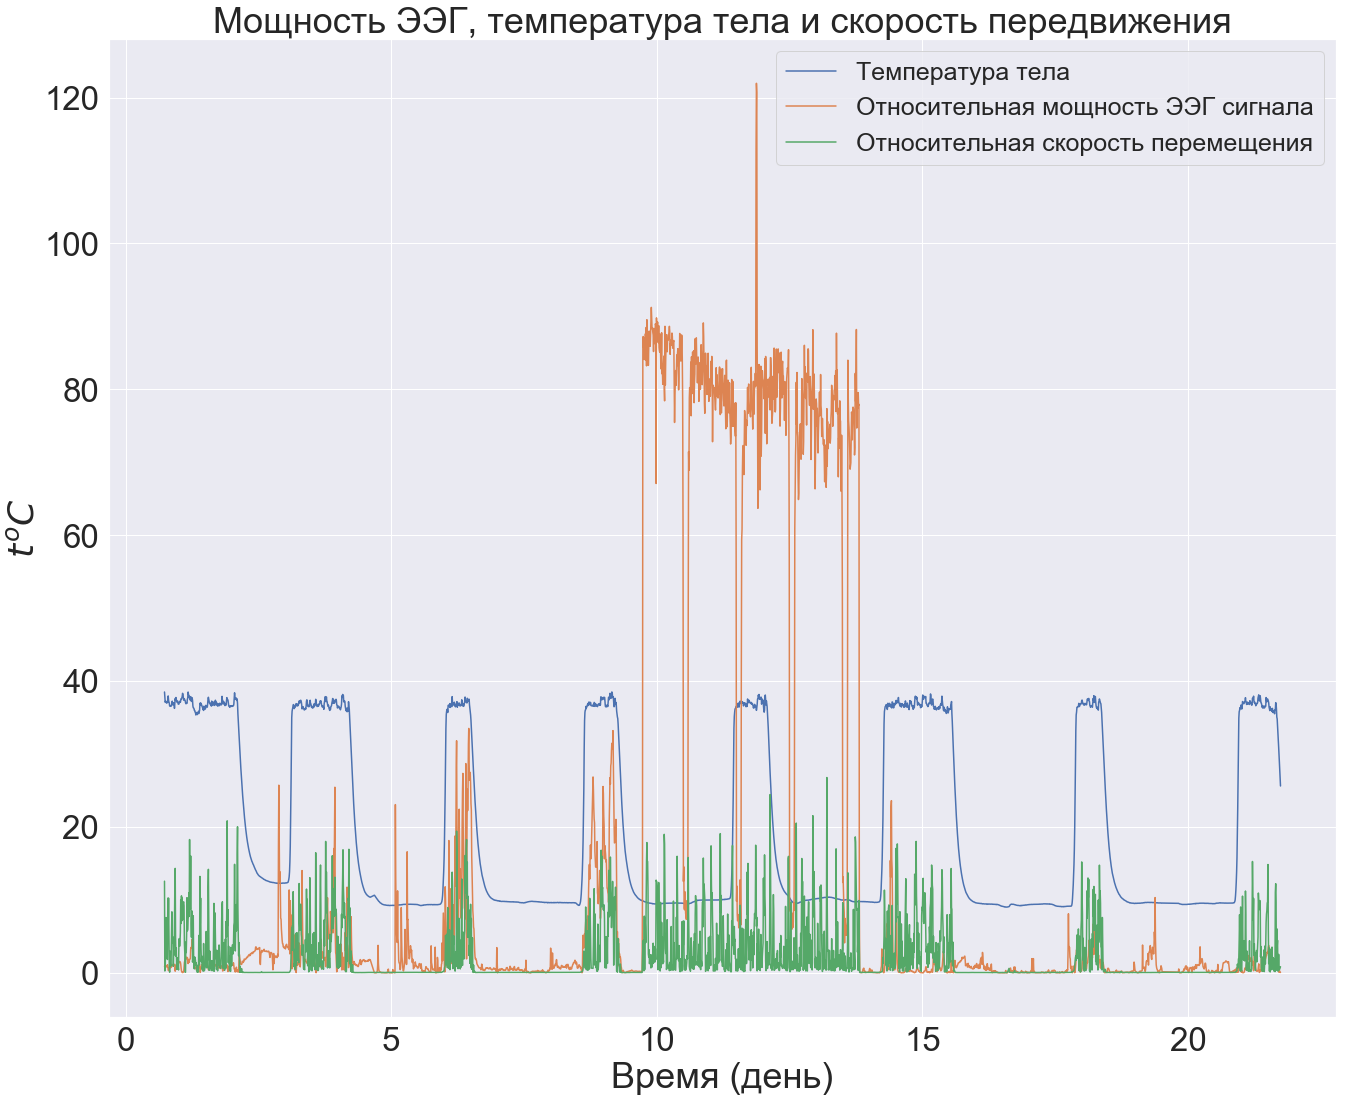
\includegraphics[width=\textwidth]{general.png}
  \captionof{figure}{На графике представлена температура тела хомяка в зависимости от времени и масштабированные значения мощность ЭЭГ, скорость. Участок с большим содержанием артефактов не удален. Представлены все полиграфические измерения.}\label{fig:general}
\end{minipage}%
\begin{minipage}{.5\textwidth}
  \centering
  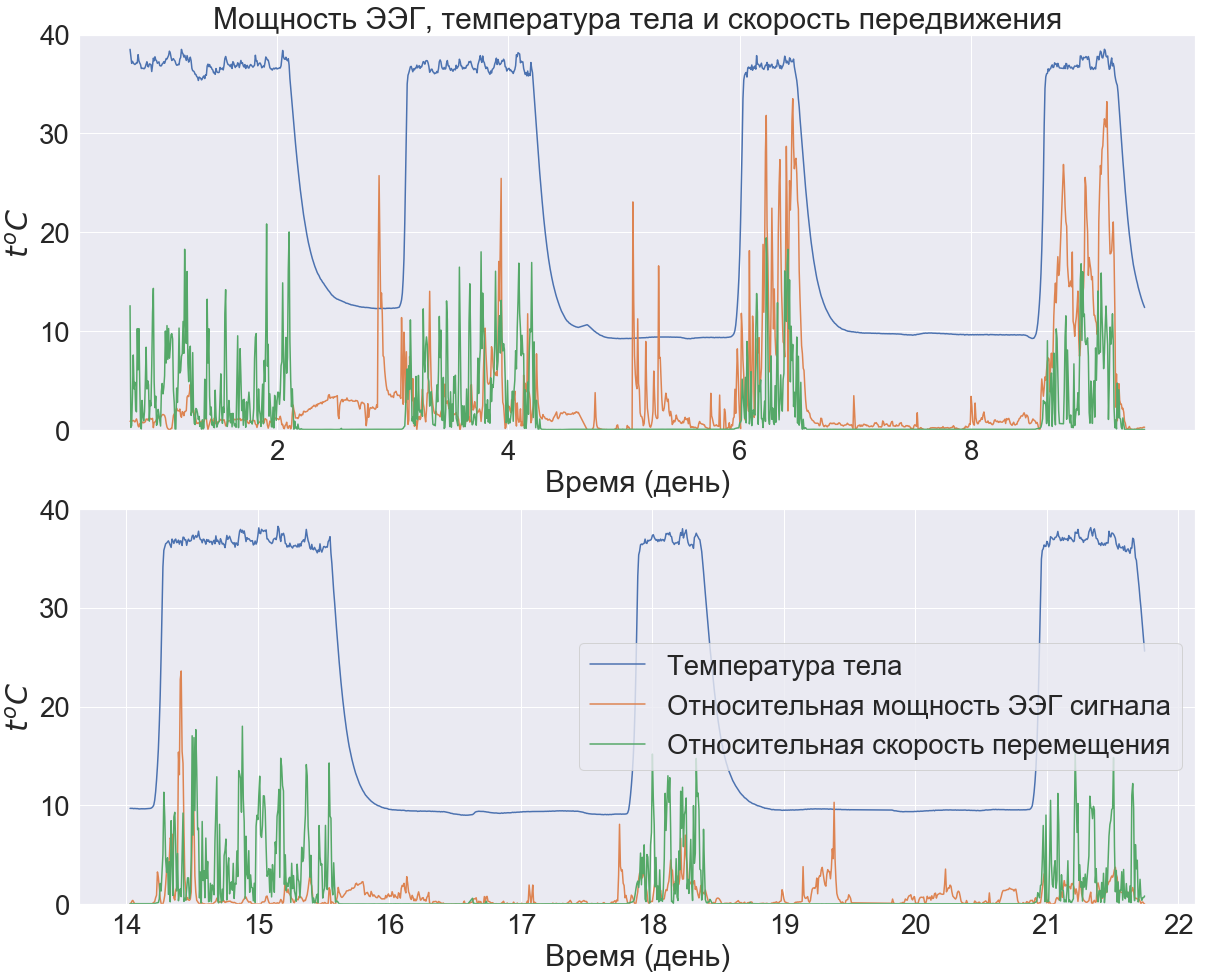
\includegraphics[width=\textwidth]{general2.png}
  \captionof{figure}{На графике представлена температура тела хомяка в зависимости от времени и масштабированные значения мощность ЭЭГ, скорость. Участок с большим содержанием артефактов, находящийся посередине, удален. График разделен на две части для удобства.}\label{fig:general2}
\end{minipage}
\end{figure}

Скорость на промежутке длинной $T$ может быть подсчитано по формуле $v_{x}(t_0, T) = \int_{t_0}^{t_0 + T} | a_{x}(t)| \; \text{d}t$. В случае физических сигналов средняя мощность на таком же промежутке подсчитывается по формуле $P(t_0, T) = \frac{1}{T} \int_{t_0}^{t_0 + T} [x(t)]^2 \; \text{d}t$. Для фильтрации был выбран устойчивый КХИ-фильтр, меньше искажающий сигнал при резких изменениях амплитуды. Артефакты, вызванные активностью, отличной от ЭЭГ, могут превышать ЭЭГ по амплитуде на короткие промежутки времени и таким образом искажать результат работы фильтров других типов.

В результате для каждой из записей были получены векторы значений скорости и мощности на 10-минутных временных интервалах, которые можно было сопоставить значениям термометра. Показания термометра, для которых не было соответствующих значений мощности и ускорения, были удалены из данных (Рис. \ref{fig:general}). В записи с 11 по 14 день наблюдается высокий всплеск мощности ЭЭГ и скорости перемещения животного. Такой сигнал сложно интерпретировать и, по всему видимому, он является продолжительным артефактом, который был удален из записи (Рис. \ref{fig:general2}, \ref{fig:general3}, \ref{fig:general4}). 

\begin{figure}[H]
\centering
\begin{minipage}{.5\textwidth}
  \centering
  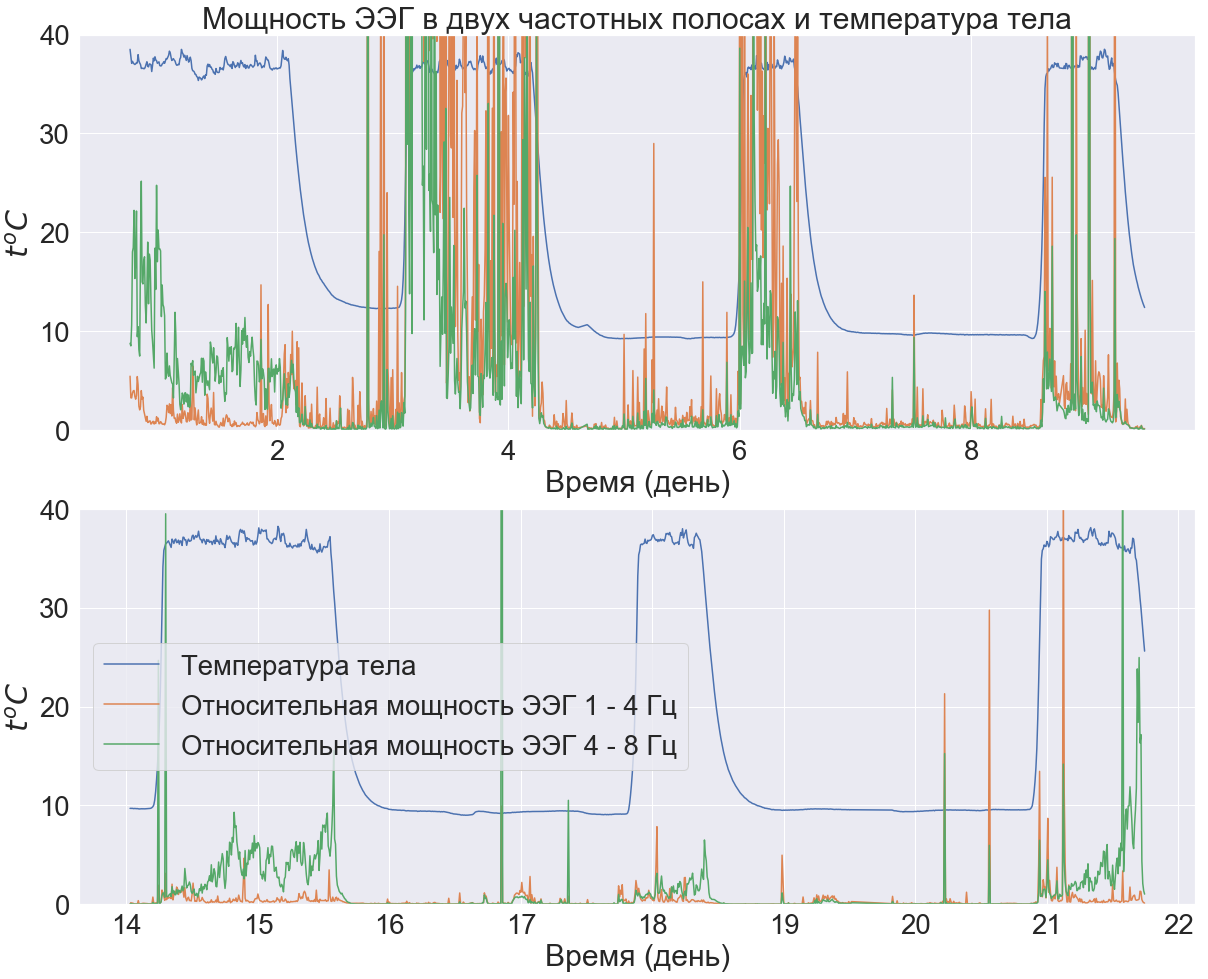
\includegraphics[width=\textwidth]{general3.png}
  \captionof{figure}{На графике представлена температура тела хомяка в зависимости от времени и масштабированные значения мощность ЭЭГ в двух разных частотных полосах (1--4 Гц и 4--8 Гц). Участок с большим содержанием артефактов, находящийся посередине записи, удален. График разделен на две части для удобства.}\label{fig:general3}
\end{minipage}%
\begin{minipage}{.5\textwidth}
  \centering
  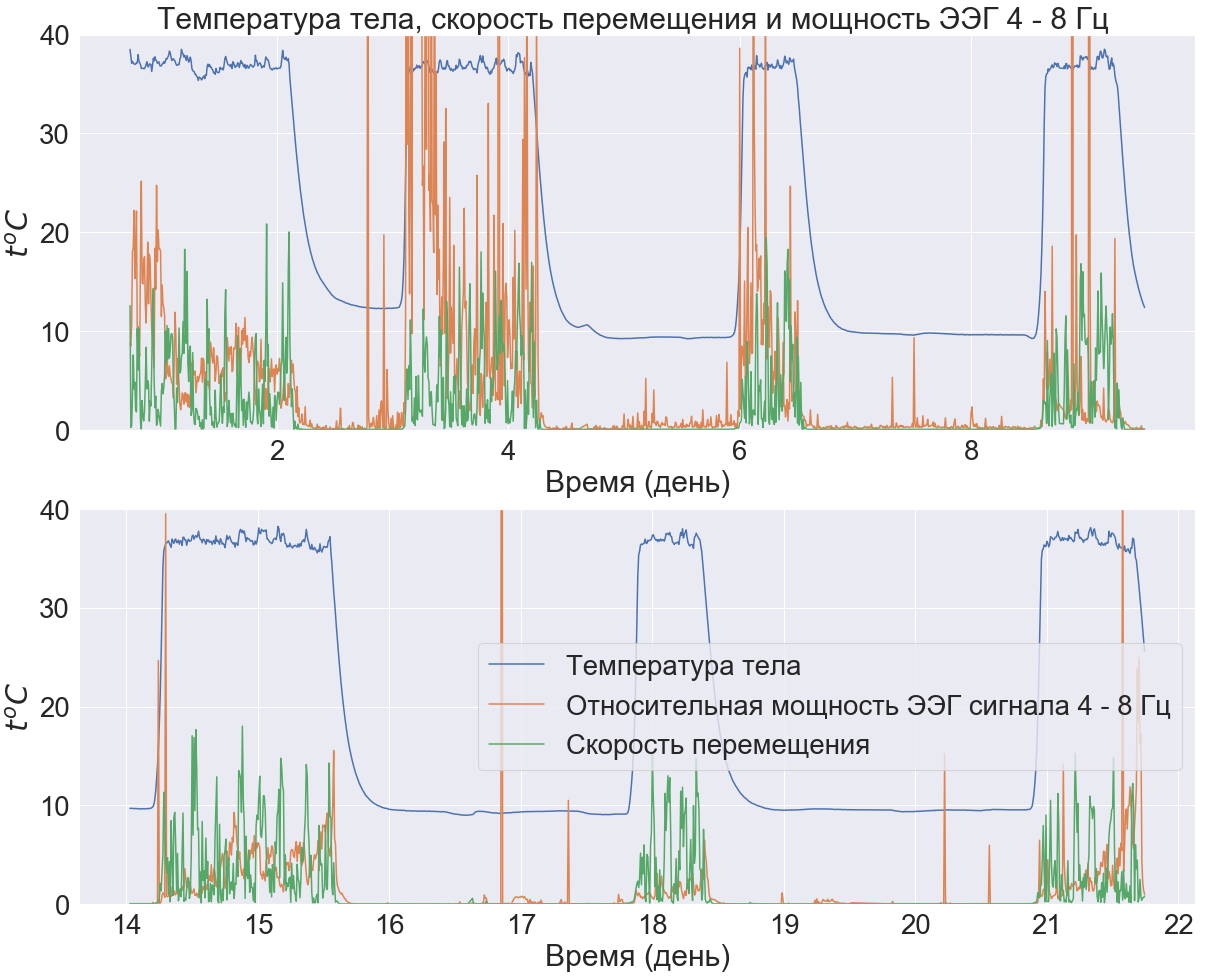
\includegraphics[width=\textwidth]{general4.png}
  \captionof{figure}{На графике представлена температура тела хомяка в зависимости от времени и масштабированные значения мощность ЭЭГ в частотной полосе 4--8 Гц, скорость. Участок с большим содержанием артефактов, находящийся посередине записи, удален. График разделен на две части для удобства.}\label{fig:general4}
\end{minipage}
\end{figure}

Когда хомяк первый раз покинул состояние торпора, значения ЭЭГ были гораздо выше, чем при бодрствовании в самом начале эксперимента. Это может значить, что выход из торпора сопровождается расходом энергии для поднятия температуры, что происходит и в нейронах и таким образом влияет на ЭЭГ. При учете того, что в конце эксперимента хомяк погиб, можно предположить, что затрата энергии при выходе из торпора привела к истощению хомяка.

\subsection{Статистика}

\begin{figure}[H]
\centering
\begin{minipage}{.5\textwidth}
  \centering
  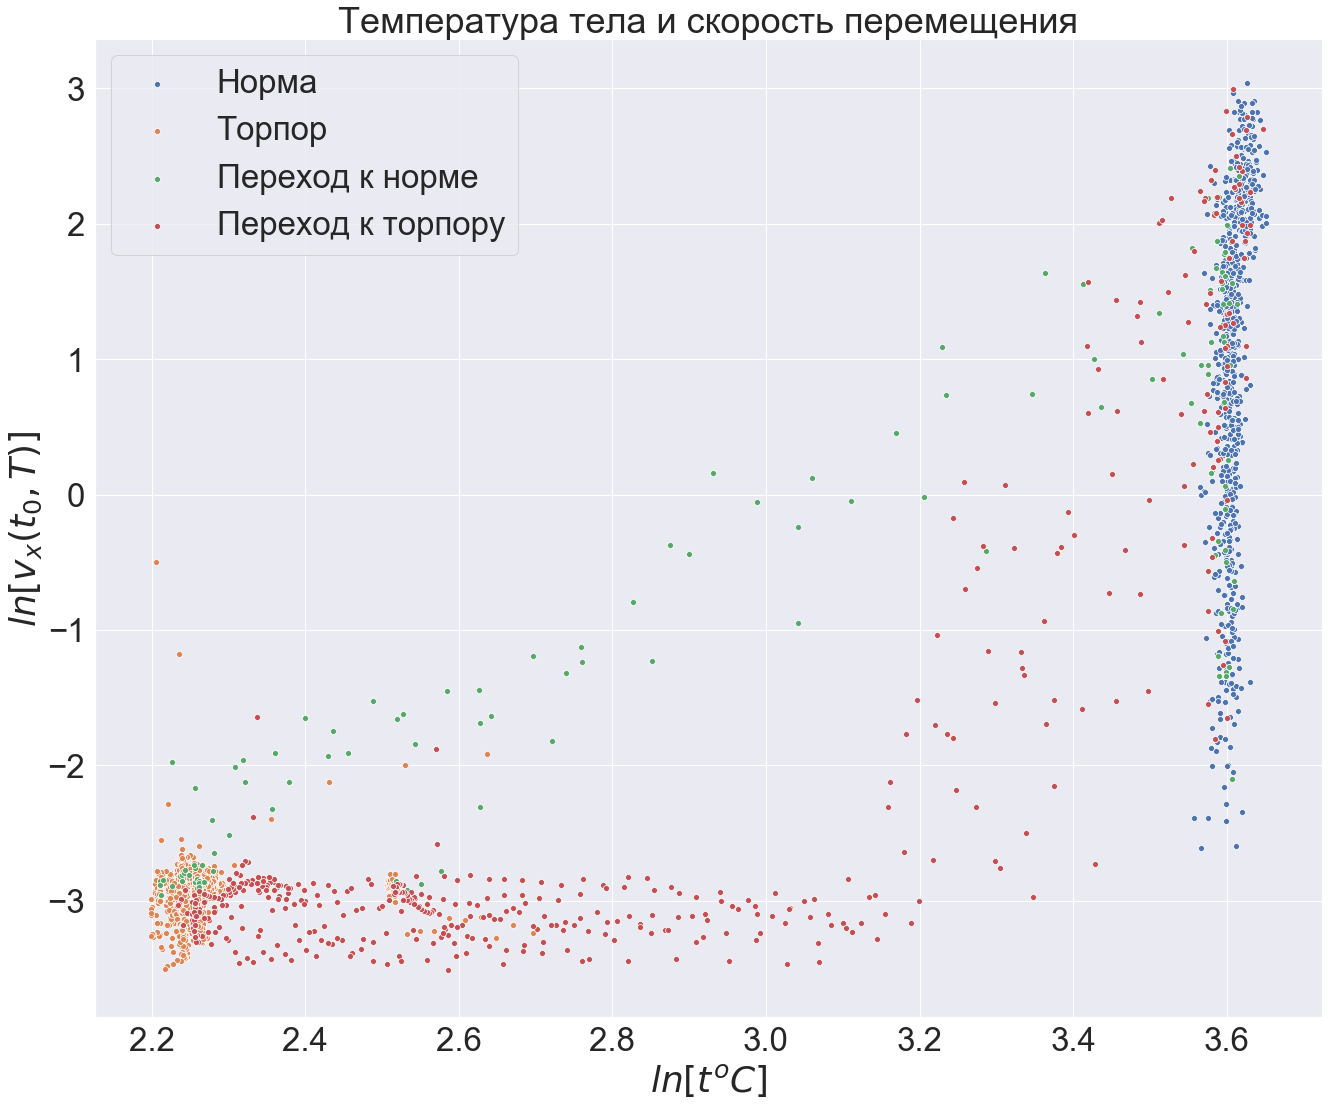
\includegraphics[width=\textwidth]{t_vs_speed.png}
  \captionof{figure}{На графике представлена диаграмма рассеяния логарифма скорости перемещения и логарифма температуры тела, позволяющая выделить четыре состояния: норма, торпор, переход к торпору и переход к норме. Состояния выделены цветами.}\label{fig:t_vs_speed}
\end{minipage}%
\begin{minipage}{.5\textwidth}
  \centering
  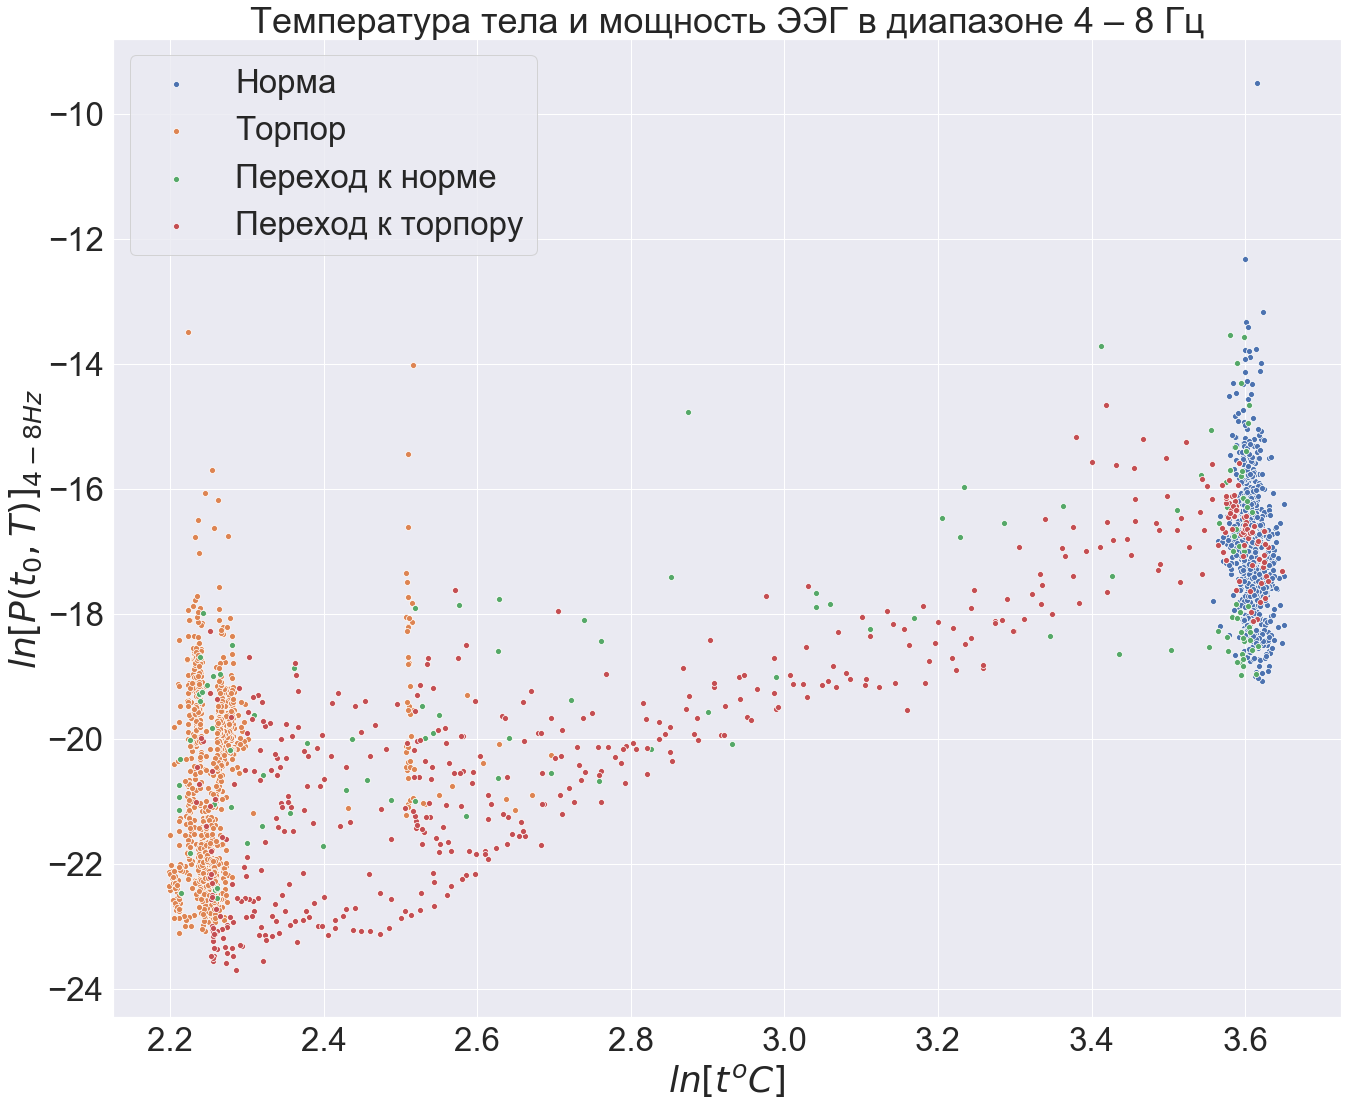
\includegraphics[width=\textwidth]{t_vs_p.png}
  \captionof{figure}{На графике представлена диаграмма рассеяния логарифма температуры тела и логарифма мощности ЭЭГ в диапазоне 4-8 Гц. На диаграмме рассеяния выделены 4 состояния, соответствующие диаграмме логарифма скорости перемещения и логарифма температуры.}\label{fig:t_vs_p}
\end{minipage}
\end{figure}

Диаграммы рассеяния позволяют выделить четыре состояния в которых мог находиться хомяк: норма, торпор, переход к торпору и переход к норме. 

Диаграмма рассеяния для температуры тела хомяка и скорости его передвижения (Рис. \ref{fig:t_vs_speed}) показывает, что скорость была ниже при низких температурах тела. Хомяк в этом случае впадал в торпор и не передвигался. При высоких температурах скорость наоборот была больше. Хомяк чаще бодрствовал и больше передвигался. При переходе от нормы к торпору видно, что хомяк останавливался и засыпал, а после этого у него начиналось понижение температуры тела. При переходе от торпора к норме видно, что скорость увеличивалась постепенно, а значит хомяк постепенно разогревался и был способен к более активному перемещению. 

Диаграмма рассеяния для температуры тела хомяка и мощности ЭЭГ в диапозоне от 4 до 8 Гц (Рис. \ref{fig:t_vs_p}) показывает, что мощность была ниже при низких температурах тела. Это можно объясняется экономией энергии в состоянии торпора. При высоких температурах мощность наоборот была больше. Хомяк бодрствовал и его мозг расходовал энергию, что приводило к электрической активности клеток. Однако, в отличии от скорости, мощность постепенно росла при выходе из состояния торпора и убывала при входе в это состояние. 

\begin{figure}[H]
\centering
\begin{minipage}{.5\textwidth}
  \centering
  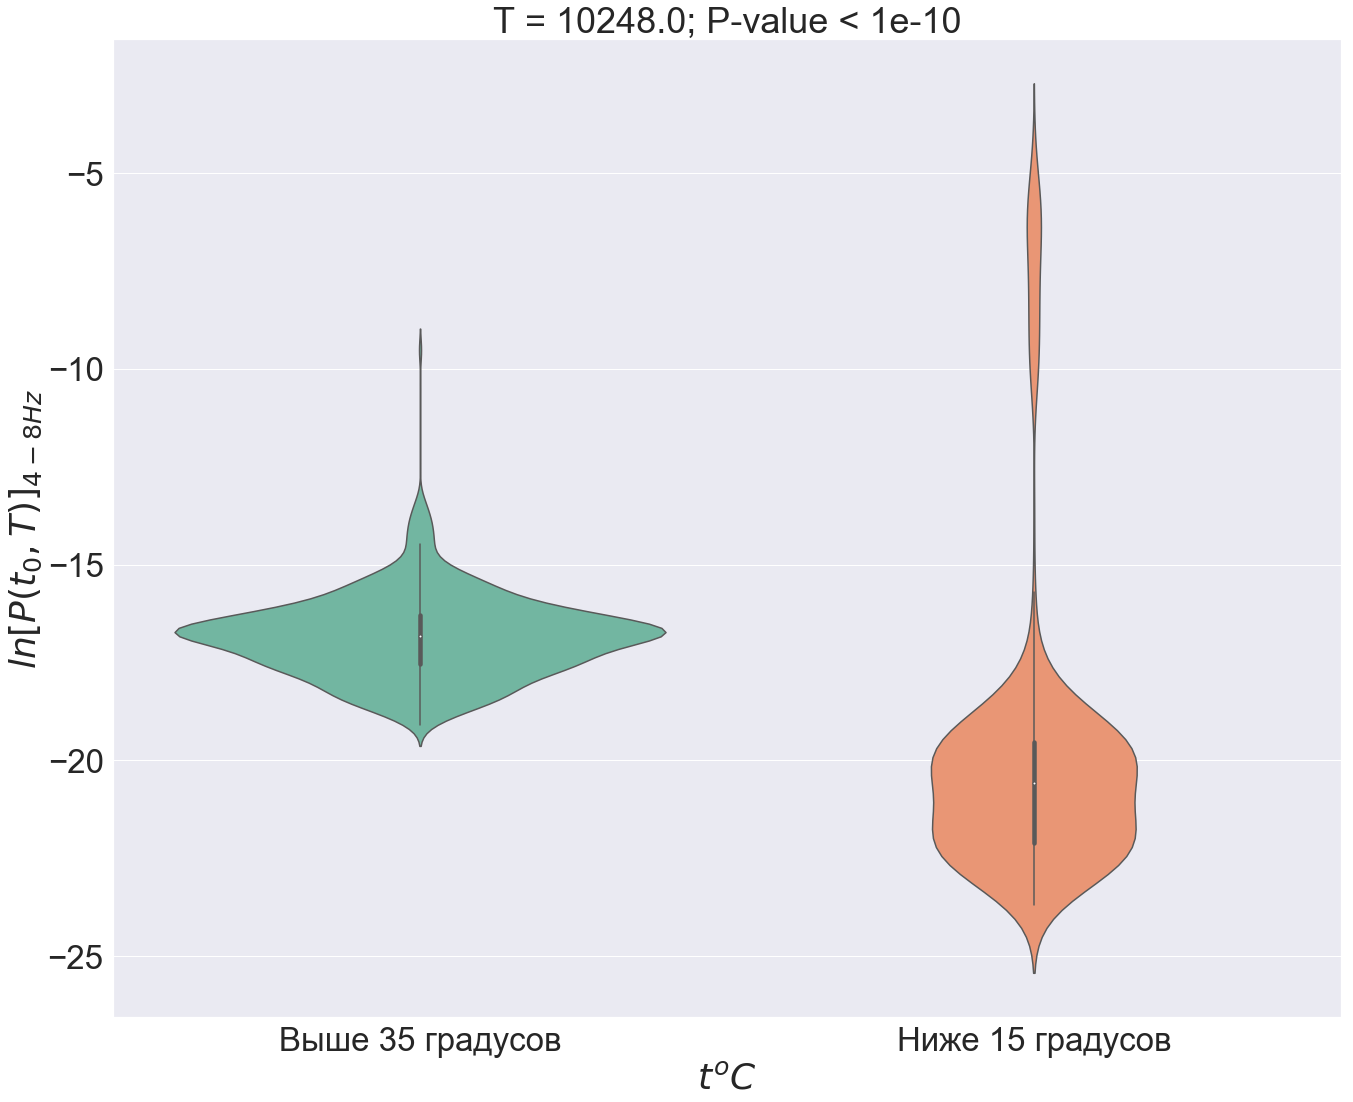
\includegraphics[width=\textwidth]{violin_plot1.png}
  \captionof{figure}{Два графика-виолончели для значений логорифма мощности при температуре выше 35 градусов и ниже 15 градусов. Над графиком приведены результаты критерия Уилкоксона.}\label{fig:violin_plot1}
\end{minipage}%
\begin{minipage}{.5\textwidth}
  \centering
  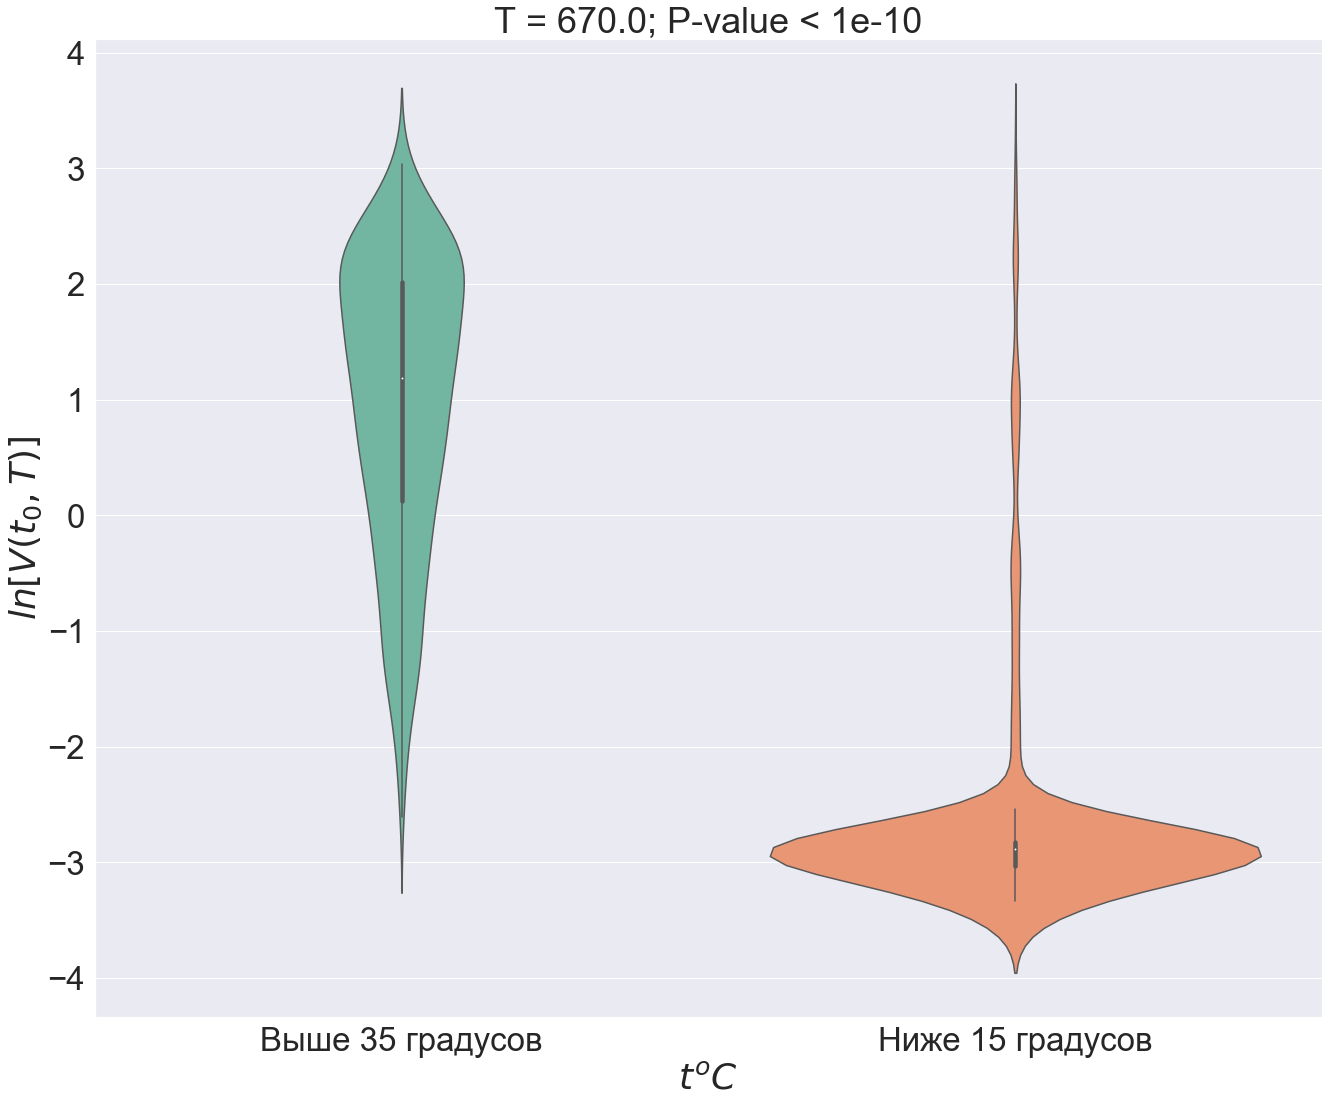
\includegraphics[width=\textwidth]{violin_plot2.png}
  \captionof{figure}{Два графика-виолончели для значений логорифма скорости при температуре выше 35 градусов и ниже 15 градусов. Над графиком приведены результаты критерия Уилкоксона.}\label{fig:violin_plot2}
\end{minipage}
\end{figure}

В зависимости от того, в каком состоянии находился хомяк, торпора или бодрствования, различия оказались значимы и между скоростью передвижения хомяка ($T = 10248$, $p < 10^{-10}$)(Рис. \ref{fig:violin_plot1}), и между мощностью ЭЭГ-сигнала в частотной полосе от 4 до 8 Гц ($T = 670$, $p < 10^{-10}$) (Рис. \ref{fig:violin_plot2}). 

\begin{figure}[H]
\centering
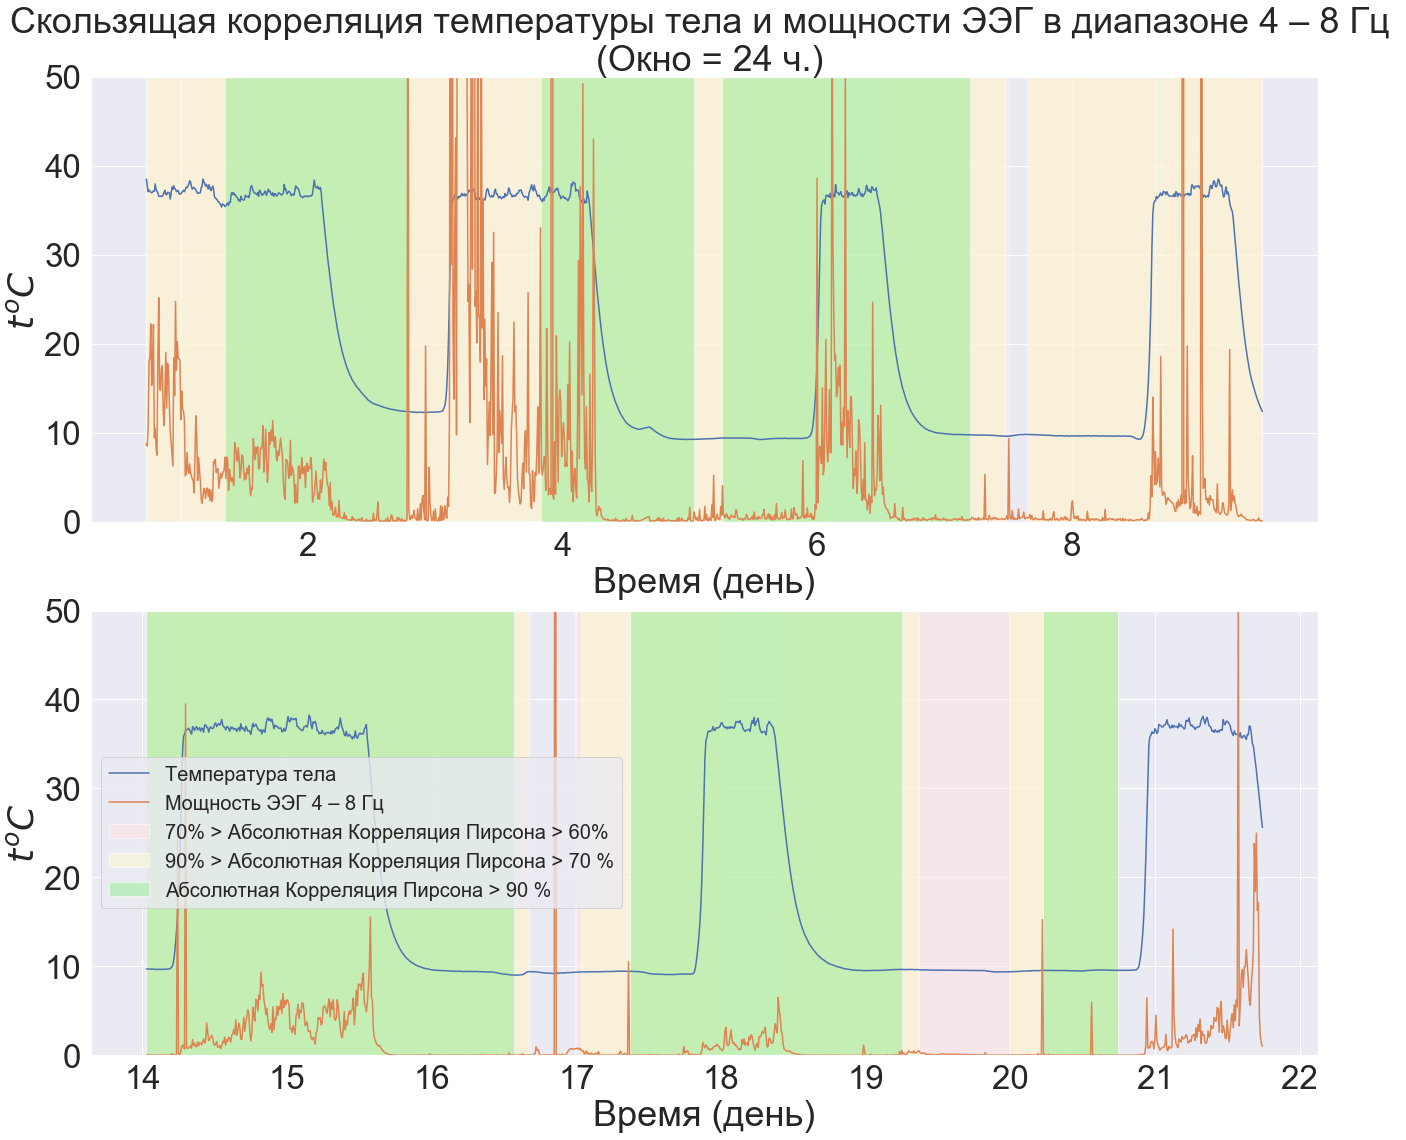
\includegraphics[width=0.7\linewidth]{moving_correlation.png}
\caption{На графике представлена температура тела хомяка в зависимости от времени и масштабированные значения мощность ЭЭГ в диапазоне от 4 до 8 Гц. Участок с большим содержанием артефактов, находящийся посередине, удален. График разделен на две части для удобства. Синим, желтым и зеленым цветами отмечены области, на которых корреляция Пирсона между логарифмом температуры тела хомяка и значениями мощности ЭЭГ достоверно значимы и имеют высокое значение. Зеленым цветом отмечены абсолютные значения корреляции больше 90\%. Желтым цветом отмечены абсолютные значения корреляции меньше 90\% и больше 70\%. Красным цветом отмечены абсолютные значения корреляции меньше 70\% и больше 60\%. }\label{fig:moving_correlation}
\end{figure}

Метод скользящего окна для корреляции Пирсона позволил установить наличие значимой корреляции логарифмированной мощности и температуры тела на разных временных интервалах проведенного эксперимента. Подробный результат представлен на рисунке \ref{fig:moving_correlation}.

\section{Приложение}

Код, выполняющий все вычисления, может быть найден \href{https://github.com/BasilMinkov/Jupyter-Notebooks/blob/master/HamsterEEG.ipynb}{в моем репозитории GitHub}. Код написан в \textbf{Jupyter Notebook} на языке \textbf{Python 3}.

\bibliographystyle{apalike}
\bibliography{/Users/wassilyminkow/Scripts/LaTeX/library.bib}

\end{document}
